\documentclass[review,times]{elsarticle}
\bibliographystyle{elsarticle-num}
\usepackage{graphicx,colordvi}
\usepackage{bm}
\usepackage{subfig}
\usepackage{xcolor}
\usepackage{listings}
\lstset{language=[08]Fortran,
  basicstyle=\small\ttfamily,
  %identifierstyle=\color{green},
  commentstyle=\color{red},
  keywordstyle=\color{blue},
  showstringspaces=false
}

\providecommand{\tabularnewline}{\\}

\begin{document}
\begin{frontmatter}

\title{LFRic: Meeting the challenges of scalability and performance portability in Weather and Climate models}

\author[met]{S.~V.~Adams}
\author[hartree]{R.~W.~Ford}
\author[met]{M.~Hambley}
\author[met]{J.~M.~Hobson}
\author[met]{I.~Kav\v ci\v c}
\author[met,read]{C.~M.~Maynard}
\ead{c.m.maynard@reading.ac.uk}
\author[met]{T.~Melvin}
\author[bath]{E.~H.~M\"{u}ller}
\author[met]{S.~Mullerworth}
\author[hartree]{A.~R.~Porter}
\author[downunder]{M.~Rezny}
\author[met]{B.~J.~Shipway}
\author[met]{R.~Wong}


\address[met]{Met Office, FitzRoy Road, Exeter, EX1 3PB}
\address[hartree]{STFC Hartree Centre, Daresbury Laboratory, UK}
\address[read]{Department of Computer Science, Polly Vacher Building,
  University of Reading, Reading, UK, RG6 6AY}
\address[bath]{Department of Mathematics, University of Bath, Bath}
\address[downunder]{Monash University, Melbourne, Australia}

\begin{abstract}
\end{abstract}

\begin{keyword}

\end{keyword}

\end{frontmatter}


\newpage
\section{\label{sec:intro}Introduction}

The Met Office develops and maintains a large suite of numerical
models that underpins its operational weather and climate research
work. At its heart is the Unified Model (UM) of the atmosphere
developed in the late 1980s and introduced into operational use in
1990~\cite{gmd-10-1487-2017}. Since its inception there has been a
continuous drive to increase the complexity, accuracy and compute
performance of the UM so as to deliver the Met Office's purpose which
is to work at the forefront of weather and climate science for
protection, prosperity and well-being.

In continuing to deliver its purpose over the next several decades,
four challenges were anticipated.

Firstly, for many years much of the improvement in compute performance
of the UM could be obtained by buying high performance computers with
ever more cores. However, clock speeds of new iterations of standard
CPUs are now often slower than the old, requiring ever more CPUs to be
used; scaling to more CPUs is limited by interprocessor
communications; and the costs of powering machines with higher core
counts is becoming ever more expensive. All these factors challenge
the ability to deliver higher resolution and more complex numerical
models~\cite{gmd-2017-186}.

Secondly, a particular challenge for many atmosphere models, including
the UM, relates to their use of the latitude-longitude (lat-lon) grid.
The convergence of longitude lines at the poles causes numerical
issues that make it hard to scale the model to higher core counts.

Thirdly, looking forward to the future, it is anticipated that HPC
architectures will change radically, and that the diversity of
architectures will increase. Even when porting from one CPU-based
machine to another, there is a cost due to the need to re-tune the
performance for the particular characteristics of the new
machine. With the emergence of more diverse machines such as GPU-based
machines, the cost will only get worse.

In collaboration with academic partners, the Met Office reviewed the
options available to resolve these three issues~\cite{GHP1_CSR}. The
decision was to develop a new model, largely from scratch, comprising
a new dynamical core written to run on an unstructured mesh that
avoided the polar singularity problem; to develop a new infrastructure
as the UM infrastructure will not support an unstructured mesh; and to
design the infrastructure with a separation between scientific code
and parallel systems code -- code that supports parallelism on HPC
machines -- so as to reduce the cost and complexity of porting to new
architectures. Furthermore, a strict API would be used so that it
would be possible to auto-generate the parallel code. This paper
describes the novel features of this new model.

The new dynamical core is called GungHo~\cite{melvin2018}. An
unstructured mesh is used whose cells are roughly equal area and which
therefore avoid the issues caused by the polar singularities of the
lat-lon grid. By employing a mixed Finite Element Method (hereafter
FEM) on an unstructured mesh, the new dynamical core is designed to
maintain the scientific accuracy of the current finite difference UM
dynamical core (ENDGame~\cite{QJ:QJ2235}).

LFRic is the name given to the new atmospheric model and underpinning
software infrastructure which are being developed to host the GungHo
dynamical core. LFRic is named after the pioneering weather forecaster
Lewis Fry Richardson. When initiating LFRic, a fourth important issue
was recognised: that while the proposed new design was novel and would
require development of new software systems, it was also important to
design a system that could use ``off the shelf'' solutions from
elsewhere if possible. For this reason, the broad design of LFRic uses
object-oriented design to modularise functionality and allow
interfacing to external packages and libraries for certain functions
such as IO and distributed memory communications.

At the core of the LFRic design, the software architecture of the
natural science code imposes a {\em separation of concerns} between
science code and code relating to parallelisation of the model. The
architecture is called PSyKAl (see Figure~\ref{fig:psykal}) after the
three layers it comprises: Parallel Systems or PSy layer code, Kernel
code and Algorithm code. The algorithm code is the top layer and is
written to operate on full model fields that represent data over the
whole domain of a global or limited area model. At the bottom, kernel
code operates on small chunks of the whole field such as a single
vertical column of data. In between, PSy layer code breaks fields down
into chunks and passes each of the chunks in turn to the kernels.

A strict API governs the implementation of the PSyKAl design,
requiring scientists to embed metadata into kernels to describe their
inputs and outputs. In effect, the API is a Domain Specific Embedded
Language (DSEL). An application called PSyclone has been developed
which interprets the embedded metadata and then generates the PSy
layer code. PSyclone can generate code that implements different
parallel strategies to target different programming models and
different system architectures. In particular, in support of current
development of the scientific model, PSyclone has successfully enabled
the LFRic model to be deployed on standard CPU based architectures through
applying distributed memory strategies and OpenMP parallelism.

The PSy layer code generated by PSyclone includes calls to the LFRic
software infrastructure. The LFRic infrastructure implements a data
model that supports finite element, finite volume and finite
difference model fields, domain decomposition of these fields on
distributed memory platforms, and halo swaps of fields to support
communication of information between distributed memory domains. This
infrastructure is implemented in Fortran and uses Fortran 2003
constructs to impose the separation of concerns.

The PSyKAl separation of concens aims to keep single source science
code separate from the complexities of the LFRic implementation. While
algorithm and kernel code is written to strict rules, it looks largely
like Fortran 90 code with minimal reference to Fortran 2003
object-orientated features. This has enabled developers to contribute
scientific code to the LFRic model with relative ease.

The paper describes the model development and is organised as follows:
The GungHo dynamical core and computational aspects are presented in
Section~\ref{sec:GH}. The software design for the separation of
concerns and PSyKAl API are described in
Section~\ref{sec:SoC}. The model infrastructure and use of libraries
is discussed in Section~\ref{sec:lib}. PSyclone, the code generator is
presented in Section~\ref{sec:psyclone} and the package developed to
apply linear solvers and preconditioners is presented in Section~\ref{sec:Solver}.
Finally a scaling analysis is presented in Section~\ref{sec:scal} and
conclusions drawn in Section~\ref{sec:con}.


\section{\label{sec:GH}GungHo}

The dynamical core in an atmospheric model is responsible for
simulating those fluid dynamical processes that are resolved by the
underlying mesh. It is then coupled to a suite of subgrid physical
parametrization schemes for processes that are not resolved (such as
cloud microphysics and convection) and those that act as subgrid
diabatic sources (such as longwave and shortwave radiative
heating/cooling). For the purposes of this paper we only consider
the dry dynamical core without the subgrid processes.

The GungHo dynamical core has been developed to replace the current ENDGame
dynamical core in the UM. The GungHo model seeks to replicate the
accuracy and stability of ENDGame whilst replacing the regular lat-lon
grid with a quasi-uniform grid and so avoid the problems associated
with the polar singularities in ENDGame, resulting from the
convergence of meridians at the poles. The mesh used in GungHo is an
equi-angular cubed-sphere, shown in Figure~\ref{fig:cubed-sphere}.
This has the benefit of near uniform resolution across the globe and a
maximum/minimum edge length of $\approx 1.3$ achieved by using only
quadrilateral cells.  However, this quasi-uniform mesh comes at the
expense of losing orthogonality (the line between two neighbouring
cells centers is not, in general, perpendicular to the edge shared
between the two cells). Additionally, the two polar singularities of
the lon-lat grid have been replaced by the eight corners of
the cubed sphere, where only three cells meet at a vertex instead of
the usual four. The lack of orthogonality and the presence of the
corner singularities need to be taken into account when choosing an
appropriate numerical method to avoid errors being dominated by the
corners.
%
\begin{figure}
\centering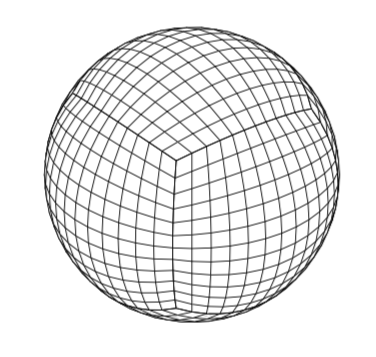
\includegraphics[width=0.6\linewidth]{Fig1_Cubed_Sphere.png}
\caption{\label{fig:cubed-sphere} Equi-angular cubed-sphere mesh as
used in GungHo with $12x12$ subdivisions per face, 
referred to as a $C12$ mesh. This gives $864$ columns of cells.}
\end{figure}
%

To generate the 3D mesh this 2D cubed-sphere mesh is extruded in the radial 
direction to form a spherical shell of cells. Where orography is present a terrain
following radial coordinate is used such that every column contains the
same number of cells. The horizontal mesh is treated as unstructured,
such that it could easily be changed, for example to one of those considered 
in~\cite{staniforth2012} such as to an icosahedral mesh.
The vertical mesh is structured and directly addressed, so that
a data point is addressed as \textit{map(df,col)+k}, where \textit{col}
is the horizontal index of the column and \textit{k=0,...,nlayers-1} is
the index of the vertical layer; \textit{df} is the index of a particular
data point within the cell, allowing multiple data points within a single cell, and 
finally \textit{map} is an array containing the address of data points at 
the bottom of the model column.
Using an extruded mesh of this type with direct access and data contiguity
in the vertical, the cost of the indirectly addressed horizontal index can 
be offset (see~\cite{gmd-9-3803-2016}) provided enough layers are used. 
Since the current UM uses~$O(100)$ layers the cost of the indirection is minimal.
%

\subsection{Formulation\label{sec:sub:formulation}}
The GungHo dynamical core solves the Euler equations for a perfect gas in a 
rotating frame
%
\begin{eqnarray}
\frac{\partial\mathbf{u}}{\partial t} & = & -\left(2\bm{\Omega}+\nabla\times\mathbf{u}\right)\times\mathbf{u} - \nabla\left(\frac{1}{2}\mathbf{u}\cdot\mathbf{u} + \Phi\right) - c_p\theta\nabla\Pi,\label{eq:momentum}\\
\frac{\partial\theta}{\partial t} & = & - \mathbf{u}\cdot\nabla\theta,\label{eq:energy}\\
\frac{\partial\rho}{\partial t} & = & - \nabla\cdot\left(\mathbf{u}\rho\right)\label{eq:continuity},
\end{eqnarray}
%
the system is closed by the equation of state
%
\begin{equation}
\Pi^{\frac{1-\kappa}{\kappa}} = \frac{R}{p_0}\rho\theta.\label{eq:eos}
\end{equation}
%
These constitute a set of coupled non-linear Partial Differential
Equations (PDEs) for the vector wind $\mathbf{u}$, 
the density $\rho$, potential temperature $\theta$ and Exner pressure $\Pi$. 
Additionally: $\bm{\Omega}$ is the rotation rate; $\Phi$ is the geopotential; 
$p_0$ is a reference pressure; $R$ is the gas constant; $c_p$ is the specific 
heat at constant pressure and $\kappa\equiv R/c_p$.

\subsection{Spatial Discretisation\label{sec:sub:spatial}}
In order to maintain a similar
accuracy to ENDGame on a quasi-uniform mesh a mixed Finite Element Method is 
used~\citep{cotter2012, natale2016}. This gives the finite element equivalent 
of the C-grid-Charney-Phillips staggering~\citep{charney1953numerical, arakawa1977computational}
used in ENDGame, but without relying
on the orthogonality of the mesh for numerical consistency. The mixed FEM
is very general in terms of the order of approximation and shape of the 
underlying mesh, allowing the method to be tailored to specific needs of the 
application. The mixed FEM involves defining a number of finite 
element spaces and differential mappings between them. The particular family of 
finite element spaces~\citep{boffi2013}, for a given polynomial order $p$, used 
in GungHo are: $Q_{p+1}$ containing continuous 
point wise scalar quantities; $N_p$ containing circulation vectors that have
continuous tangential components; $RT_p$ containing flux vectors that have 
continuous normal components; $Q_p^D$ containing discontinuous volume 
integrated scalars; along with a horizontally discontinuous vertically continuous 
space~\citep{natale2016} for $\theta$ to mimic the Charney-Phillips grid staggering 
used in ENDGame. Here continuous means that neighbouring cells share degrees of freedom 
(hereafter dofs) located on the shared entities (e.g. faces, edges, vertices).
In practice the lowest order spaces $p=0$ are used, the resulting location of the dofs
for these spaces are shown in Figure~\ref{fig:fem-spaces}. 
%
\begin{figure}
\centering
\subfloat[]{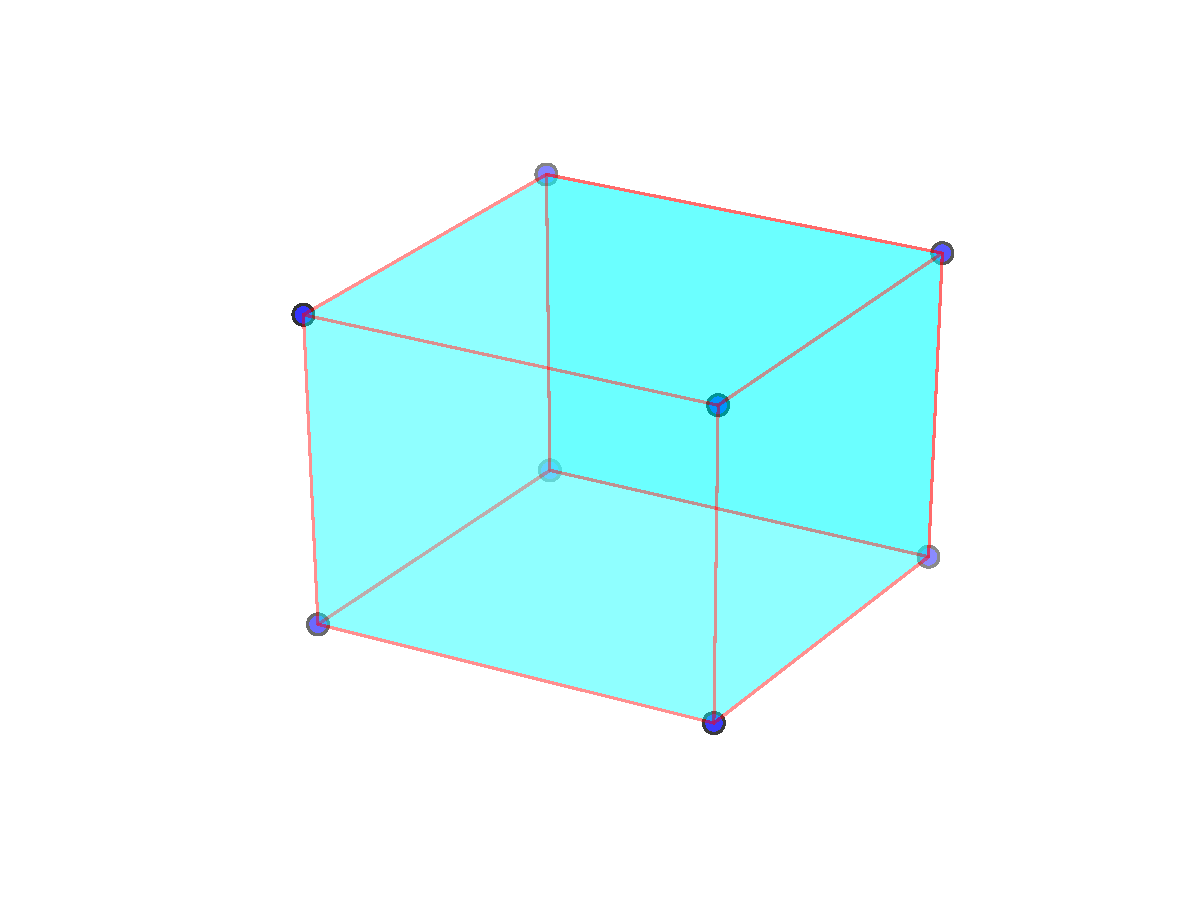
\includegraphics[width=0.5\linewidth]{Fig2a_W0_dofs.pdf}}%
\subfloat[]{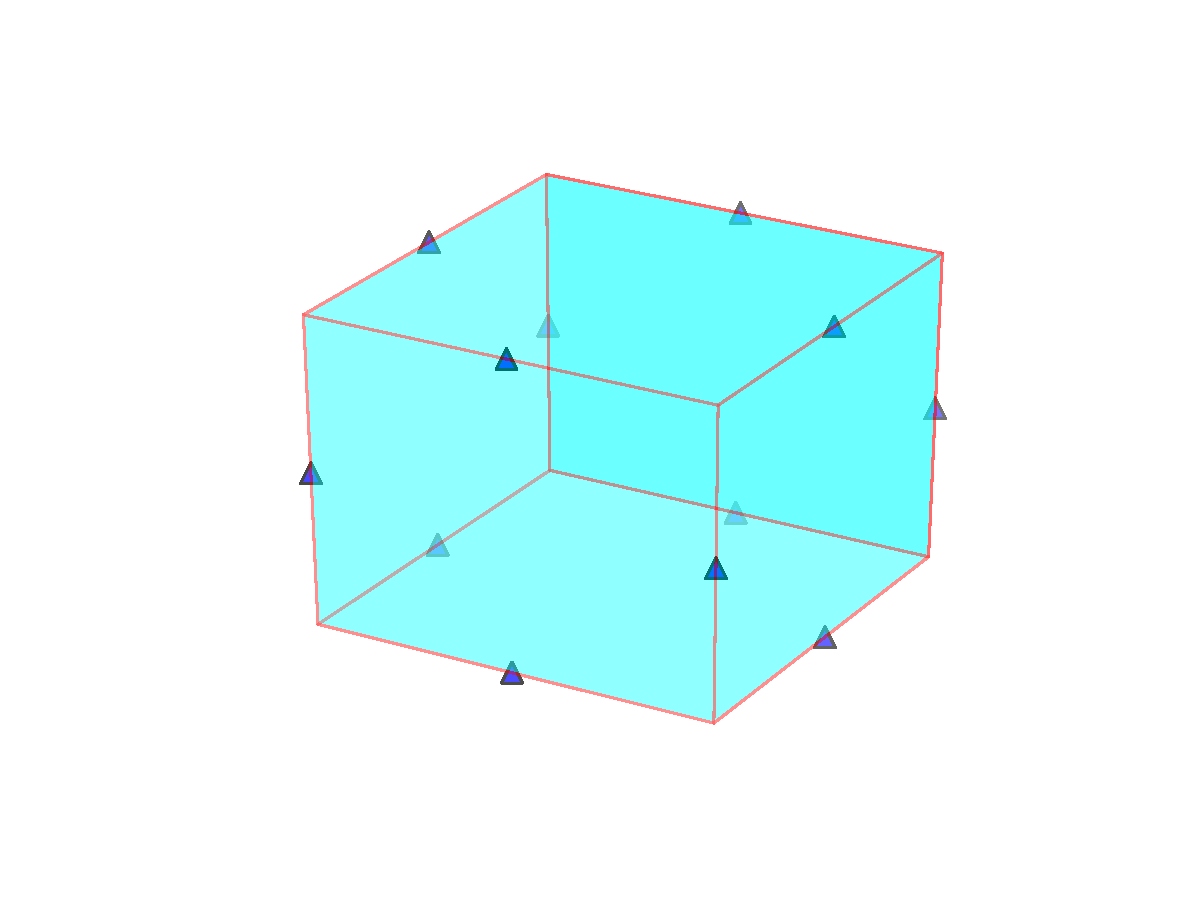
\includegraphics[width=0.5\linewidth]{Fig2b_W1_dofs.pdf}}\\
\subfloat[]{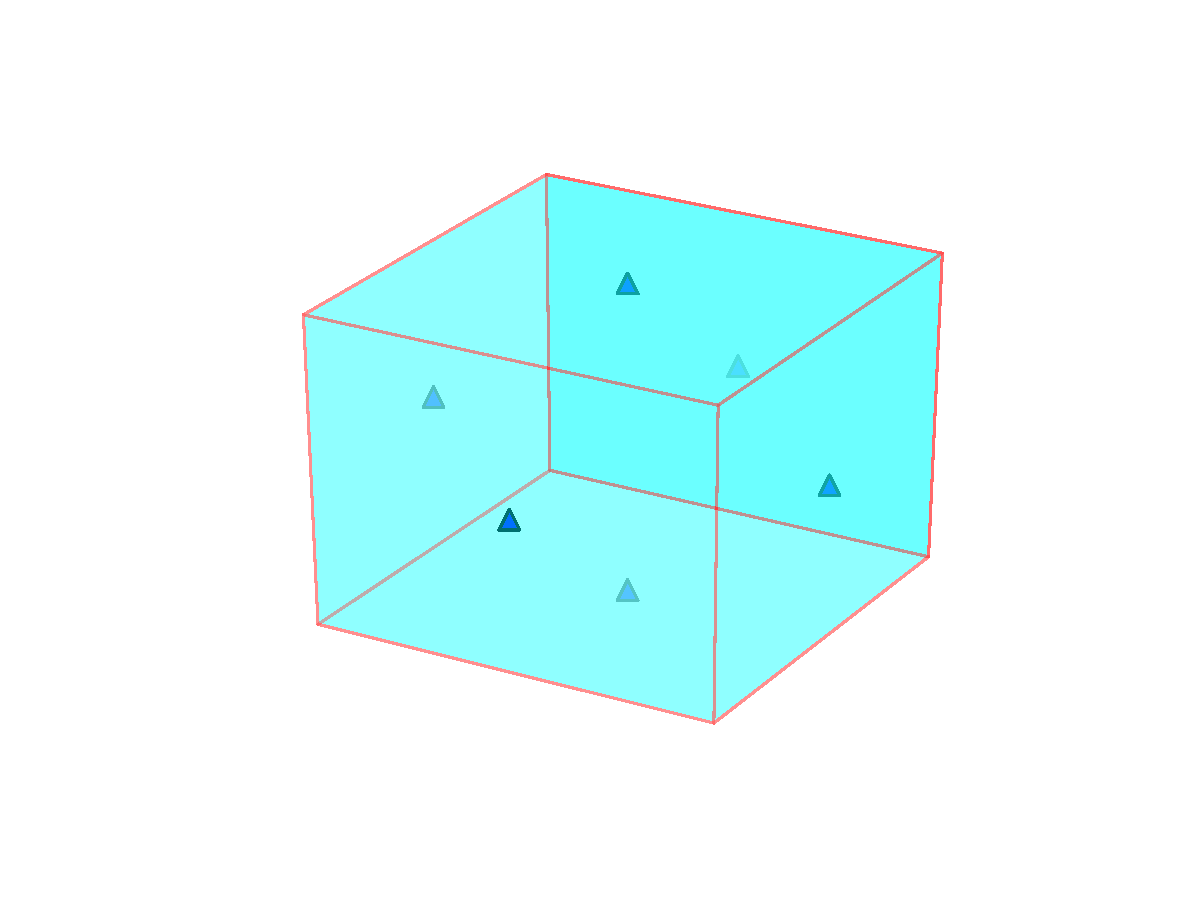
\includegraphics[width=0.5\linewidth]{Fig2c_W2_dofs.pdf}}%
\subfloat[]{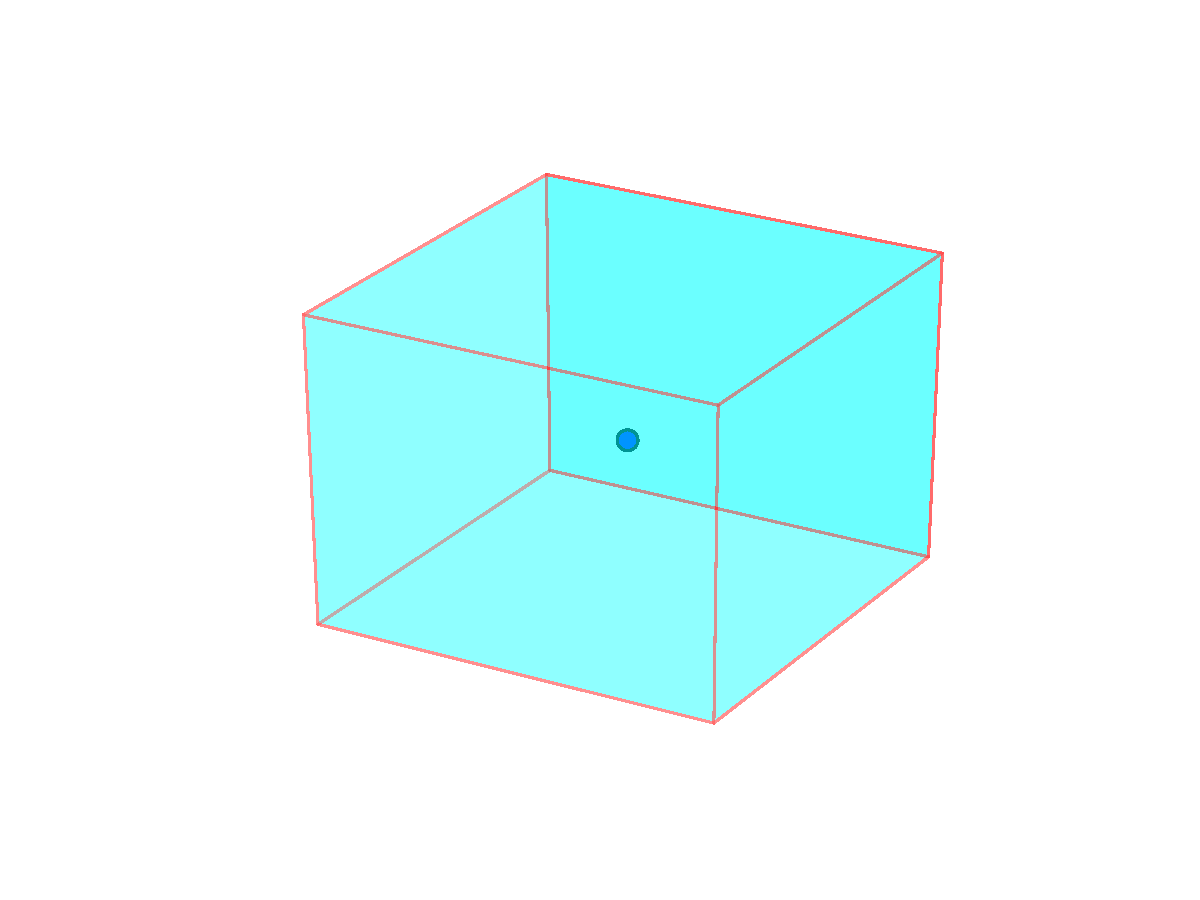
\includegraphics[width=0.5\linewidth]{Fig2d_W3_dofs.pdf}}%
\caption{\label{fig:fem-spaces} Location of degrees of freedom at $p=0$ for 
(a) $Q_{1}$, (b) $N_0$, (c) $RT_0$ and (d) $Q_0^D$ finite element spaces.
Circles correspond to scalar degrees of freedom and triangles to vector degrees
of freedom.}
\end{figure}
%
The velocity field $\mathbf{u}$ is placed in the $RT_0$ space; the vorticity 
$\xi\equiv\nabla\times\mathbf{u}$ is placed in the $N_0$ space; density, $\rho$, 
and Exner pressure, $\Pi$, are placed in the $Q_0^D$ space; as mentioned above 
the potential temperature, $\theta$, is placed in a scalar-space corresponding 
to the vertical components of $RT_0$ with dofs located in the
centre of the top and bottom faces of a cell. See~\cite{melvin2018} for a full
description of the discretisation used in the GungHo model.

\subsection{Advection\label{sec:sub:advection}}
In order to achieve accuracy similar to that of ENDGame it is important to have 
a high-order approximation to the scalar advective terms: $\mathbf{u}.\nabla\rho$ 
and $\mathbf{u}.\nabla\theta$. In ENDGame these are evaluated using a 
semi-Lagrangian formulation that involves computation of the trajectories that 
the fluid has taken over a timestep, followed by a high-order multi-dimensional 
interpolation of the scalar field to the origin of the trajectory. 
The non-local nature of the trajectory computation can 
lead to significant communication costs if the trajectory crosses over processor 
boundaries, which often happens near the poles of the lat-lon grid.

In GungHo this semi-Lagrangian scheme is replaced by an Eulerian finite-volume 
method of lines advection scheme that gives inherent local conservation of mass.
The method fits a high-order upwind polynomial over a number of
neighbouring cells and evaluates this at a fixed point to compute the advective 
term. This only requires a local computation and the stencil is fixed, reducing the 
amount of computation needed. However, in order to obtain a stable scheme it is 
wrapped in a multi-stage evaluation, meaning that the advection update needs to be 
computed a number of times per iteration of the iterative-semi-implicit scheme
(see Subsection~\ref{sec:sub:timestepping}), nominally 3 stages are used. 
Future work will evaluate the use of flux-form Semi-Lagrangian scheme (COSMIC)~\cite{Leonard1996} 
to replace the current scheme. This carries many of the 
benefits of the semi-Lagrangian scheme used in ENDGame but without the 
communication costs (due to use of a quasi-uniform mesh) as well a simplification 
to the computation from using a dimensionally split formulation that only requires 
one-dimensional interpolation.

\subsection{Time-stepping\label{sec:sub:timestepping}}
As in ENDGame, to facilitate the use of long time-steps, a two time-level 
iterative semi-implicit time-stepping scheme is used. This requires, within each 
time-step, a non-linear Picard iteration to update the non-linear and advection terms 
and at each iteration a large sparse linear system is solved, which is formed by 
use of a quasi-Newton method,
%
\begin{equation}
\mathcal{L}\left(\mathbf{x}^n\right)\mathbf{x}' = \mathcal{R}\left(\mathbf{x}^{(k)}\right),\label{eq:quasi-newton}
\end{equation}
%
for the increment $\mathbf{x}'\equiv\mathbf{x}^{(k+1)}-\mathbf{x}^{(k)}$ on the $k^{\rm{th}}$ 
estimate from the Picard iteration of the prognostic variables $\mathbf{x}\equiv\left(\mathbf{u},\,\theta,\,\rho,\,\Pi\right)$. 
The linear system $\mathcal{L}\left(\mathbf{x}^n\right)$ is chosen as to contain the terms necessary for stability of 
the fast acoustic and gravity waves as in~\cite{QJ:QJ2235} and is formed from a linearisation about the previous 
timestep fields $\mathbf{x}^n$. The method used to solve this linear system is detailed in Section~\ref{sec:Solver}. 
An overview of the time-step is given in Table~\ref{tab:timestep}.
%
\begin{table}
\begin{centering}
\begin{tabular}{l}
\hline 
\textbf{do} $n=1,N$ (begin time-step loop)\tabularnewline
\hspace{0.5cm}Set $\mathbf{x}^{(1)} = \mathbf{x}^n$\tabularnewline
\hspace{0.5cm}Compute $\mathcal{L}\left(\mathbf{x}^n\right)$\tabularnewline
\hspace{0.5cm}Compute $R\left(\mathbf{x}^n\right)$\tabularnewline
\hspace{0.5cm}\textbf{do} $k=1,K$ (begin Picard loop)\tabularnewline
\hspace{1.0cm}Compute advective terms $R^A\left(\mathbf{x}^{(k)},\mathbf{x}^{(n)}\right)$\tabularnewline
\hspace{1.0cm}Compute $R\left(\mathbf{x}^{(k)}\right)$\tabularnewline
\hspace{1.0cm}Set $\mathcal{R}^{(k)} = R^n + R^{(k)} + R^A$\tabularnewline

\hspace{1.0cm}Solve $\mathcal{L}\left(\mathbf{x}^n\right)\mathbf{x}' = \mathcal{R}^{(k)}$\tabularnewline
\hspace{0.5cm}\textbf{end do}\tabularnewline
\hspace{0.5cm}Set $\mathbf{x}^{n+1} = \mathbf{x}^{(K)}$\tabularnewline
\textbf{end do}\tabularnewline
\hline
\end{tabular}
\end{centering}
\caption{\label{tab:timestep}Overview of a single timestep in the GungHo dynamical core, typically $K=4$.}
\end{table}
%

\section{\label{sec:SoC}Separation of Concerns}
Science applications in general and weather and climate codes in
particular are written in high-level languages such as Fortran or
C/C++. Indeed, Fortran is commonly employed for weather and climate
codes and can be considered a Domain Specific Language (DSL) for
numerical computation. Using such a high-level language, an
algorithm is written to solve a mathematical problem without
consideration for the processor architecture. The compiler generates
machine specific instructions and can, in principle, make optimisation
choices to exploit the architecture of different processors.

This abstraction of a separation of concerns between mathematics code
and machine code is powerful and enables both the portability of
science code to different processor architectures and allows the
application to exploit a significant\footnote{What constitutes good
performance depends on a variety of factors.} fraction of the peak
performance of the processor. Whilst many science applications may
contain code optimisations in performance critical sections (for
example, blocking or tiling loop nests to better utilise cache memory),
in general these applications have relied on clock
speed increases between processor generations to increase performance.

Increases in processor speed between generations ceased more than a decade
ago due to the absence of Dennard scaling~\cite{dennard}. Instead,
successive generations of processors have had increasing numbers of processor cores per
socket. Science applications typically have already been adapted to run on multiple
nodes to exploit supercomputers with the distributed memory and data parallelism
typically expressed over MPI. However, multi-core nodes present
additional challenges and heterogenous compute nodes such as
CPU + GPU with distinct memory spaces require additional programming
models. Moreover, the algorithms employed combined with data
parallelism may not be sufficient to exploit this explosion of parallelism.

A great number of programming models exist. For distributed memory there are, 
for instance, MPI and Partitioned Global Address Space (PGAS) languages, such 
as Co Array Fortran, Unified Parallel C, Chapel and GASPI. For threaded and 
shared-memory parallelism there are directive-based solutions such as OpenMP 
and OpenACC as well as languages such as CUDA and OpenCL. However,
the programming models lag behind in development of the rapidly evolving computer
architectures and particular models lack feature or processor coverage
making the choice of programming model difficult. This is ambiguity is
especially difficult for weather and climate applications with their long development
cycles. 

Many applications have adopted an MPI + X model, where X is one or
more of the programming models mentioned in the previous paragraph. This
is problematic for several reasons. The programming models are not
only different, they are different types of model. Languages, language
extensions, libraries and directives, some of which are architecture
specific. Worse, the interaction between them is outside the scope of
any model\footnote{Whilst MPI has some level of threaded awareness,
  this is limited.} and may, for example, require the batch scheduling
system to control this. The applications may require a different X for
different architectures and even different data layouts and
loop nest order. All these parallel and performance features
break the data abstraction of the separation of concerns between the
maths/science code and architecture specific code.

The design for the LFRic model is based upon a computational science
report from Phase 1 of the GungHo project~\cite{GHP1_CSR}. By
employing a layered software architecture, the complex parallel code
can be kept separate from the science code. As outlined in 
Section~\ref{sec:intro}, the software is separated into three layers.
Algorithms are expressed as operations on global, data-parallel field objects,
in the top algorithm layer. The middle PSy layer (Section~\ref{sec:intro}) 
contains the horizontal looping and is where the data parallelism is expressed. 
The bottom layer is comprised of the kernels which encode the operation invoked in the
algorithm layer. These are chosen to operate on a single column of data. 
Shown in Figure~\ref{fig:psykal} is a schematic diagram of this
layered software achitecture. The red arrows indicate the control flow
through the different layers. 

\begin{figure}
\centering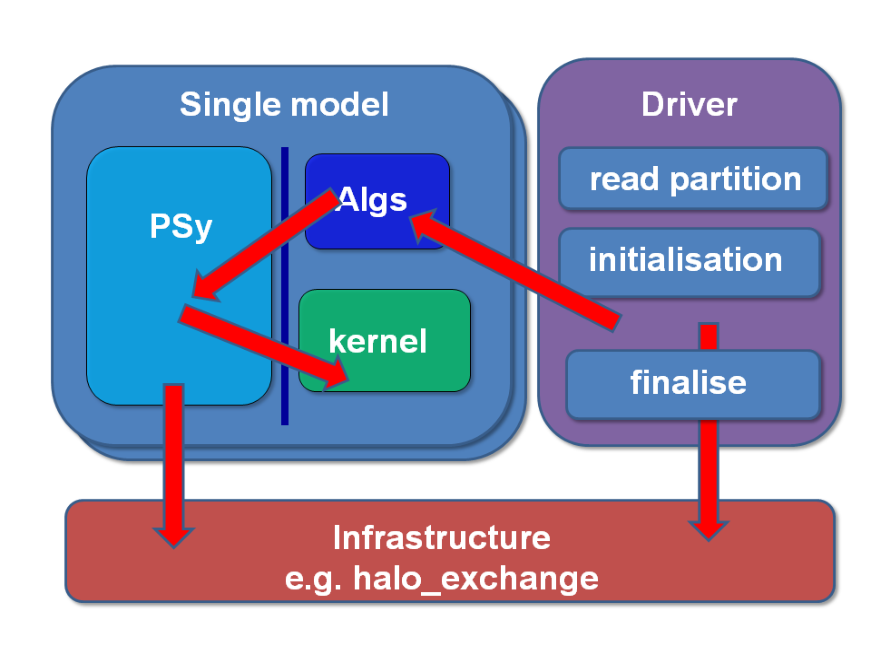
\includegraphics[width=0.8\linewidth]{Fig3_PSyKAl.pdf}
\caption{\label{fig:psykal} Schematic diagram of the PSyKAl layered
  architecture. A single model could be for example, the atmospheric
  model. The blue vertical line between the PSy layer and the
  Algorithm and Kernel layers represents a separation of the science
  and parallel code.}
\end{figure}

The APIs between the layers are tightly controlled. The PSy layer can
only be called from the algorithm layer by an {\em invoke} procedure
call. The permitted arguments to these invoke procedures are restricted
to be the kernels and the fields that the kernels will operate on. The
kernels can only be called from the PSy layer with the unpacked data
arrays, scalars for loop bounds and supporting arrays of both reals
and integers for the Finite Element Method over the horizontally unstructured mesh.
These coding rules are enforced by using Fortran 2003 object
orientation coding style to control the APIs. By restricting the
domain of the problem from all numerical mathematics to only that
required (in the first instance) in the GungHo dynamical core it is
possible to constrain the parallelism to the PSy layer. Restoring
the separation of concerns between the science code and the
parallel/optimisation code means that in principle different programming
models can be employed in the PSy layer without changing the science
code. Moreover, the PSyKAl API can be thought of as a Domain Specific
Embedded Language (DSEL).

Compilers in general have to be conservative about the assumptions
they can make in order to guarantee correctness. However, a further
advantage of the domain specific approach is that developers can
explicitly express the domain knowledge which is not possible in a
standard, high level language. In the case of the LFRic model, data
access descriptors are employed to say whether access to a field is
{\em read}, {\em write}, {\em readwrite} or {\em increment}. The latter 
two discriminate between fields that do not share degrees 
of freedom between columns ({\em e.g.} density defined on 
$Q_p^D$ function space, see Subsection~\ref{sec:sub:spatial} for more details) 
and the ones that do ({\em e.g.} velocity defined on $RT_0$ space, 
Subsection~\ref{sec:sub:spatial}). This information is embedded in
Fortran as part of the kernel. Other information encoded in this way
is the loop iterator (for example, the choice to loop over horizontal {\em cells}), whether the kernel
operates on a field which lives on a specific function space, whether
any of the fields live on common function spaces and for FEM kernels
whether the kernel uses any basis functions. 

The restricted domain, strict control of the APIs between layers and,
critically, the data access descriptors and other kernel metadata
allow the PSy layer to be constructed entirely according to a set of
rules. The code itself can then be automatically generated. This is
done by a Python code parser, transformer and code generator called
PSyclone. More details of PSyclone itself can be found in
Section~\ref{sec:psyclone}. The generated code is mostly Fortran.
These are calls to the LFRic infrastructure (see Section~\ref{sec:lib} 
for more details) which might contain the
MPI distributed memory parallelism and infrastructure calls
to dereference the Fortran 2003 objects, looping over
the horizontal mesh elements and calling the kernels
themselves. However, PSyclone can also perform transformations and
target other progamming models such as OpenMP or OpenACC. PSyclone is
then in effect a Domain Specific Embedded compiler. PSyclone also does
one other important code generation function; In the algorithm layer,
the calls to the invoke procedure are replaced with a specific
procedure call to the PSy layer. The PSy layer code can then be
optimised depending on the kernels in the invoke and the metadata.

\subsection{\label{sec:sub:implement}Implementation}
The algorithm layer code is written in Fortran 2003. However, this
code is not actually compiled, it is parsed and processed by PSyclone
first. Most of the Fortran is left as written. The exception to this
is the call to any {\em invoke} procedure. The invoke procedure does not 
exist as such in the source code. Instead, an invoke means {\em execute these
kernels looping over the chosen entities}, hence instructing PSyclone on how to 
generate parallel code. PSyclone can paralellise this horizontal looping with MPI,
OpenMP or both. Shown in the code fragment below is an invoke
procedure call from the algorithm layer.

\begin{lstlisting}[language=Fortran,caption={Code fragment showing an
invoke procedure from the Algorithm layer},label={lst:invoke}]
 call invoke(setval_c(v(m), 0.0_r_def), &
             matrix_vector_kernel_type(v(m), s(m), mm), &
             enforce_bc_kernel_type( v(m) ) )
\end{lstlisting}

There are three kernels in this invoke. The first \verb+setval_c+ is
an example of a {\em point-wise} kernel. The same operation, setting all
the values of the field to the same scalar, is applied to each dof so no 
FEM structure is required. This is an example of a {\em built-in} operation 
generated in place in the PSy layer by PSyclone. The second
kernel is written as a call to the constructor of the kernel type, so that it is
valid Fortran. The arguments to this call \verb+v+ and \verb+s+ are
{\em fields} and \verb+mm+ is an {\em operator}, in this case a mass
matrix.

PSyclone replaces the code for an invoke to the kernels with a call to a
generated procedure in the PSy layer, with the fields and operators as
arguments. This is shown below
\begin{lstlisting}[language=Fortran,caption={Code fragment showing the
generated Algorithm layer code},label={lst:invoke_56}]
 CALL invoke_56(v(m), s(m), mm)
\end{lstlisting}

Shown in listing~\ref{lst:PSy1} is a code fragment from the generated PSy layer for
the invoke shown in listing~\ref{lst:invoke}.

\begin{lstlisting}[language=Fortran, numbers=left,caption={Code 
fragment of the generated PSy layer},label={lst:PSy1}]
 CALL v_proxy%set_dirty()
 CALL v_proxy%halo_exchange(depth=1)
 IF (s_proxy%is_dirty(depth=1)) THEN
   CALL s_proxy%halo_exchange(depth=1)
 END IF 
 DO cell=1,mesh%get_last_halo_cell(1)
   CALL matrix_vector_code(cell, nlayers, v_proxy%data, &
      s_proxy%data, mm_proxy%ncell_3d, mm_proxy%local_stencil, &
      df_any_space_1_v, undf_any_space_1_v, &
      map_any_space_1_v(:,cell), &
      ndf_any_space_2_s, undf_any_space_2_s, &
      map_any_space_2_s(:,cell))
  END DO 
  CALL v_proxy%set_dirty()
  CALL v_proxy%halo_exchange(depth=1)
\end{lstlisting}
Lines 1-20 are the calls to the LFRic infrastructure to extract
sizes, loop counters, and the indirection maps for the unstructured
mesh. Lines 24-26 are the built-in function generated in place in the
PSy layer for a point-wise operation. Lines 30-36 are the distributed
memory calls to the infrastructure for a halo exchange and
testing/setting flags to indicate whether a halo (and to what depth)
has been updated. Lines 38-45 are the looping over the horizontal mesh
and the procedure call to the kernel itself. The arguments are simple
scalars for sizes and loop counters, the data arrays and (in this example)
the indirection maps. 


Shown in the code fragment below is the kernel metadata for the
matrix-vector kernel invoked in the algorithm layer.
\begin{lstlisting}[language=Fortran, numbers=left,caption={Code
fragment showing kernel metadata for the matrix-vector operator kernel},label={lst:metadata}]
type, public, extends(kernel_type) ::  &
                    matrix_vector_kernel_type
  private
  type(arg_type) :: meta_args(3) = (/ &
       arg_type(GH_FIELD,    GH_INC,  ANY_SPACE_1), &
       arg_type(GH_FIELD,    GH_READ, ANY_SPACE_2), &
       arg_type(GH_OPERATOR, GH_READ, ANY_SPACE_1, &
       ANY_SPACE_2)  /)
  integer :: iterates_over = CELLS
contains
  procedure, nopass ::matrix_vector_code
end type
\end{lstlisting}
The metadata is embedded in Fortran so that no special comments or
other mark-up is required. The access descriptors shown above are key
to deriving the appropriate rules for generating the code in the PSy
layer. The \verb+arg_type+ has three components. Firstly, the type of
the data object, in this case fields and operators\footnote{An
  operator is a mapping between one function space and another.}. Secondly, what is
the data acess pattern for this data object, {\em e.g.} \verb+GH_INC+ means the data is
incremented. Thirdly, which function space the data lives on. In this case, the
kernel is general and can operate over any space, hence, the
\verb+any_space_n+. Whilst the $n$ can be any number, the function space of the
first field must correspond to the first function space of the operator and the
function space of second field must correspond to the second function
space of the operator. 


\section{\label{sec:lib}Infrastructure}

As shown in Figure~\ref{fig:psykal}, the PSyKAl layered
architecture is supported by the LFRic infrastructure. This provides
functionality such as distributed memory support (halo exchanges),
colouring for OpenMP threading and the provision of loop bounds that the
generated PSy layer will use.

\begin{figure}
\centering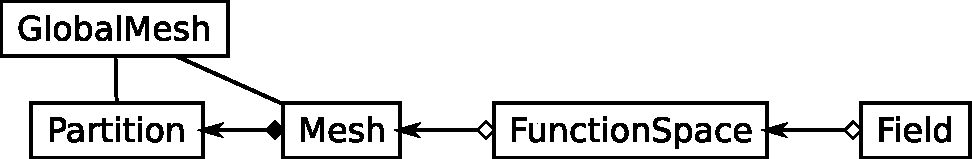
\includegraphics[width=0.8\linewidth]{Fig4_FieldClass.pdf}
\caption{\label{fig:objects} A Unified Modelling Language (UML) 
class diagram of the family of objects used
in the LFRic infrastructure to support the field object.}
\end{figure}

Within the development of LFRic there has been a conscious effort to
provide the infrastructure following an object-orientated approach. As
such, much of the infrastructure is provided through a family of
objects that ultimately support the field object that is used within the
science code. The objects are shown in
Figure~\ref{fig:objects}. Two-dimensional topological and positional
information about the global mesh is read into the global model object.
This is passed to a partitioner to generate a partition object that
describes what portion of the global mesh the local processing element
will be working on. The global mesh and the partition objects are then
combined to form a mesh object that extrudes the two-dimensional mesh
information in the vertical for just the part of the mesh that will be
used on the local processing element to form a local, three-dimensional
representation of the mesh. The way the data that is held within the
field object relates to the mesh is described by the function space.

Most of the infrastructure is accessed through the field object. So, for
example if a halo exchange is required on a field, the halo exchange
method on the field object is called. This infrastructure
API is used by the PSy layer to access information and functionality.

\subsection{\label{sec:sub:distmem}Distributed Memory Optimisation}

Distributed memory parallelism is achieved by partitioning the full
(global) domain into smaller sections (partitioned or local domains).
Information is passed between the tasks through the use of halo regions.
Data in these areas are provided from other partitions that own that
section of the domain.

Performing halo exchanges is not unique to LFRic. Running large parallel
weather and climate model codes has been done for many years, using
halo exchanges as a
method of providing communication between partitions. The LFRic
infrastructure has a data model with significant differences to previous
models which will affect the way distributed memory parallelism is
implemented:

\begin{enumerate}

\item LFRic is designed to support horizontally unstructured meshes,
which means it has to support non-uniform shaped partitions with complex
shaped halo regions;

\item Because the domain is horizontally unstructured, moving from one
data point to a horizontally adjacent data point requires using a lookup
table, which is slower than using direct addressing. In order to recover
some code performance, fields are laid out in memory so that vertically
adjacent data points are next to each other, which means that, for
optimisation reasons, the looping structure within LFRic is vertical
looping innermost;

\item LFRic supports a finite-element formulation which means that data
are held as dofs on all the different
entities within the mesh: cell volumes, faces, edges and vertices.
Partitioning the domain along cell boundaries will always lead to
partitions which need to share data values. Sharing data makes assigning
ownership of that data, and therefore, halo swapping more complex.

\end{enumerate}

The halo exchanges are achieved by passing information between processes 
using MPI. For performance and ease of use reasons, the MPI library is not 
called directly, instead a layer between the model and MPI is introduced. 
At initialisation time, the layer is responsible for pre-generating the 
communication routing tables required to perform a halo exchange, which 
are then reused every time a halo exchange is required.

In order to generate the routing table, each rank needs to supply the
following information to the library:

\begin{itemize}

\item A list of all the global dof ids of all the locally owned dofs;

\item A list of all the global dof ids of all the dofs in the halos.

\end{itemize}

Initially, the LFRic project used the infrastructure library component
of the Earth System Modelling Framework (ESMF)~\cite{ESMFDocs} to
provide the layer between the model and MPI, however it was not particularly
well suited to the particular problem it was being used for. Although
routing tables it generated were optimal (the halo exchanges called
during timestepping were very fast), the time to generate the tables
became quite long when the model was run at scale. The design of the
model framework to support the `separation of concerns' led to all the
halo exchange functionality being neatly encapsulated in the PSy layer.
This made it relatively easy to try a different library to provide the
intermediate layer. A switch was made to use the YAXT (Yet Another
eXchange Tool)~\cite{YAXTDocs} library. This provides
halo exchanges during time stepping that are as fast as those provided
by ESMF, but the time taken to initialise the routing tables is much
shorter.

The API for supporting distributed memory optimisation is very simple. A
halo exchange function is provided on every field and a flag is
maintained by the infrastructure to track whether data held in the halo
cells is up to date with the owner of that data (`clean' halos) or
whether a parallel computation has updated the field on the owning
partition and the local halos are out of date (`dirty' halos). When the
PSy layer determines that a halo exchange may be required, it first
checks the state of the halos and if (and only if) they are `dirty' it 
calls the halo exchange functionality.

\subsection{\label{sec:sub:sharedmem}Shared Memory Optimisation}

As with all the parallelisation within LFRic, the shared memory
parallelism is implemented within the PSy layer. The directives that
control the shared memory parallelism are inserted into the PSy layer
code. The finite element formulation makes use of data on mesh entities
shared by more than one cell. Two different threads working on
adjacent cells may try writing to a dof shared between the cells at the
same time.
{\em Graph colouring} is applied to the mesh so that no cells of any one
colour share dofs. This means parallel threads can run over the whole
set of cells within a particular colour and safely write dof values
without contention.
The information and functionality to support
colouring within the shared memory parallelism is provided by the LFRic
infrastructure.

When the mesh object is created, it is coloured by the infrastructure
and information about the colouring is stored, so it can be used from
within the PSy layer. The infrastructure provides the number of colours,
the number of cells in each colour and which cells are present in each
colour. Shared memory parallel directives are placed in the PSy layer
and the looping can be made safe using the colouring information
provided by the infrastructure. 

\subsection{\label{sec:sub:io}Parallel I/O}

A consequence of models running over many thousands of cores is a requirement
for scalable parallel I/O. A computationally optimised model is of little practical
operational use if I/O then becomes a limiting factor. The LFRic project has
decided to investigate options for I/O alongside the computational
and infrastructure development for three main reasons. Firstly, the requirement
to be able to run science assessment jobs on large numbers of cores and obtain the
output efficiently. Secondly, a key aim of LFRic is scalability and therefore it is
helpful to be able to monitor the impact of I/O on this as the infrastructure and
science develops. Thirdly, LFRic is making some fundamental changes that impact the
underlying mesh and this links to I/O in terms of input/output file formats. Having
a concrete idea of what these file formats will be in the future enables LFRic to
inform future users, internal and external to the Met Office.

Although developing a bespoke I/O system was a possibility, the decision was
made early on to adopt an existing parallel I/O framework and leverage knowledge and
experience from the community; developing Earth System Models is becoming increasingly
complex and challenging for any one organisation to develop and maintain all the required
components~\cite{gmd-2017-186}.
As of early 2016, when the first scoping work for LFRic parallel I/O was being done,
there were several existing parallel I/O frameworks and XIOS was selected as the prime
candidate for evaluation~\cite{XIOSWiki}. A discussion of the other frameworks and why
they were not considered can be found in~\cite{Adams2018}.

XIOS was an obvious choice for LFRic as it was a mature framework, having had many years
of development and was already in use in the weather and climate domain; for example,
the Orchidee land surface model, the Dynamico dynamical core (part of the LMD-Z
Atmosphere model) and the NEMO ocean model. NEMO is used in Met Office coupled
models so there was some existing experience with XIOS. In terms of potential scalability,
XIOS had also been proved to run successfully in models running on the order of 10,000
cores. Crucially for climate models, XIOS works with the OASIS coupling framework that
is commonly used in coupled climate models including the UM. 

The key features of XIOS can be summarised as follows:
\begin{enumerate}
  \item Flexible definition of I/O workflows via external XML files;
  \item Client/Server architecture allowing asynchronous I/O servers on dedicated cores;
  \item Sophisticated "in situ" post-processing via workflows defined in the XML file(s). 
\end{enumerate}

XIOS is written in C++, but also provides a Fortran API to developers. It makes use of
MPI-IO and the NetCDF4 and HDF5 libraries and handles unstructured and regular grids.
XIOS is a client-server framework where I/O servers are asynchronous processes buffering
output requests from client processes. XIOS also has sophisticated post-processing
functionality - {\em e.g.} for regridding, time series, meaning. The output schedule and
file format are defined by an XML file which hides a lot of complexity from the user.

Prior to 2016, XIOS only supported read and write of NetCDF file formats that follow the CF
conventions.  As previously explained in Section~\ref{sec:GH}, the LFRic implementation uses
semi-structured meshes and a FEM formulation, where variables are held on
different elements of the mesh (vertices, edges or faces). Therefore, the I/O system needs to
handle data structured in this way. The UGRID-NetCDF format has been chosen as the main
LFRic input mesh format and also output format for diagnostics and model dumps~\cite{UgridSpec}.
In the UGRID convention the topology of the underlying unstructured mesh is stored as well as
data, and data can be defined on any of the mesh elements: vertices, edges, or faces.
Working in collaboration with IPSL (Institut Pierre Simon LaPlace), the ability to write the
UGRID format was added to XIOS in 2016 in order to support LFRic. 

XIOS has been integrated into LFRic via a lightweight I/O interface so
that (as far as possible) the underlying I/O framework is hidden and
could be replaced by an alternative.  The I/O interface is designed to
be compatible with the use of Fortran 2003 Object Orientation in
LFRic. The field object (see Figure~\ref{fig:objects}) contains read and write
interface declarations that use Fortran procedure pointers to define
I/O 'behaviours'. When a field is created the behaviours are set by
pointing to a specific reading or writing method. Writing a field just
involves calling \verb+field%write_field()+ - {\em i.e.}, it is the
responsibility of the field to write itself and how the writing is
actually done is hidden.

More details of the experimental results of the LFRic-XIOS integration work can be
found in~\cite{Adams2018} where preliminary results on I/O scalability (up to 13824 
processors) and XIOS and Lustre performance tuning are presented. The conclusions of
this work were that XIOS is an effective parallel I/O framework that was technically
straightforward to integrate into the existing LFRic infrastructure via the XIOS
Fortran interface. Scaling experiments showed that XIOS performance was scaleable with
respect to increasing numbers of cores, even with minimal tuning.

\section{\label{sec:psyclone}PSyclone}

As discussed earlier, PSyclone~\cite{psyclone} is a domain-specific
compiler which, given an Algorithm and associated Kernels, generates
the code for the middle, PSy layer. Currently, each of these layers
must be in Fortran and hence the compiler is embedded in
Fortran. The choice of Fortran is motivated in Section~\ref{sec:SoC}. However, there is
nothing in the approach to prevent other languages being targetted in
future. PSyclone itself is written in Python.

Figure~\ref{fig:psyclone-arch} shows the data flow within the PSyclone
architecture.  Starting from the left, the Algorithm is parsed (using
fparser, a pure Python implementation of a Fortran parser) and any
invoke procedure calls identified. The list of kernels (and their arguments)
associated with each of these calls is then stored. For each invoke,
the Fortran modules containing the kernel code (as identified by
the Fortran use statements) are parsed and the meta-data for each kernel
extracted.

\begin{figure}
\centering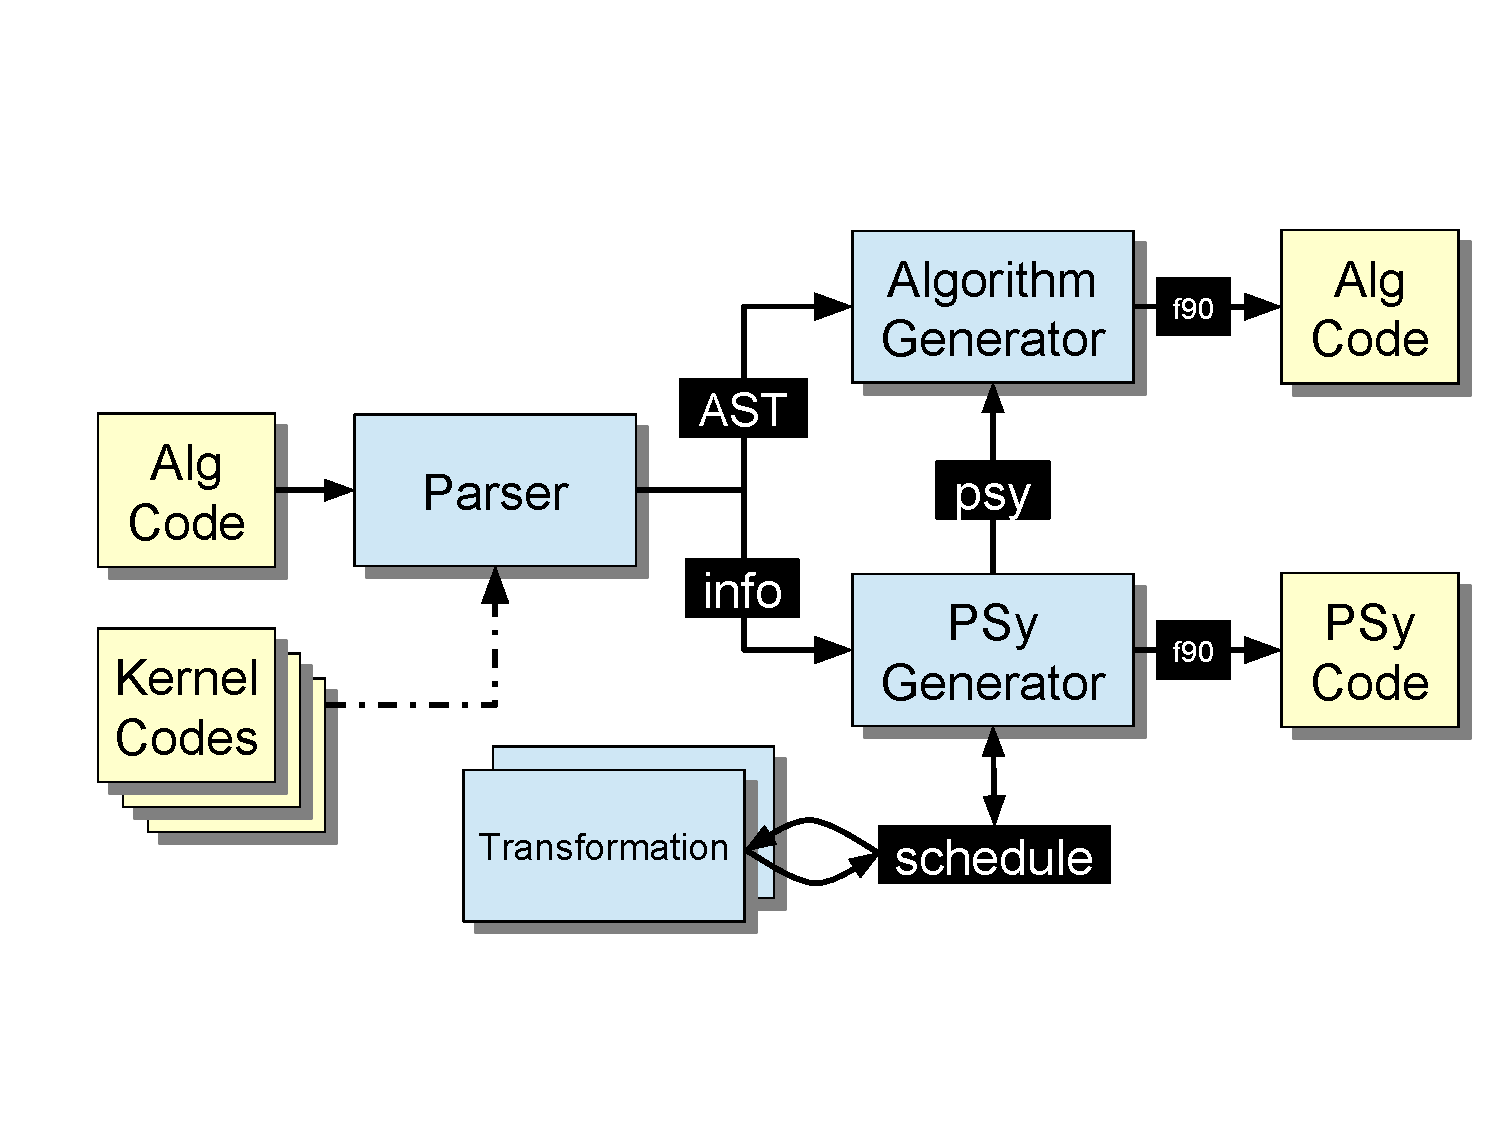
\includegraphics[width=0.8\linewidth]{Fig5_psyclone_flow.pdf}
\caption{\label{fig:psyclone-arch}Data flow within the PSyclone architecture.}
\end{figure}

PSyclone must then perform two tasks: firstly, generate an internal
representation, known as a {\em schedule}, of a PSy layer routine for each invoke in
the Algorithm. If distributed memory is specified then this schedule
must include appropriate halo exchanges and global sums to ensure
correct execution. Secondly, PSyclone must modify the supplied Algorithm
code and replace each `call invoke' with a call to the corresponding
routine in the PSy layer. This latter task is achieved by modifying
the fparser-produced Abstract Syntax Tree (AST) of the Algorithm and
then re-generating Fortran from the new AST.

If no transformations are being applied (see below) to the PSy layer
schedule(s) then all that remains is for the PSy generator to create
Fortran code.  The steps involved in generating a vanilla
(un-optimised) PSy layer subroutine are as follows:
\begin{enumerate}
\item Generate the unique list of arguments required by all kernels
  in the invoke;
\item Generate Fortran which queries the LFRic infrastructure to get
  information on the sizes of the various iteration spaces (number of cells,
  vertical levels, dofs {\em etc.});
\item Generate Fortran which queries the LFRic infrastructure to get the
  various look-up tables ({\em e.g.} for identifying the dofs belonging to a
  given cell);
\item Generate Fortran which dereferences the various field and operator
  objects to get the necessary data arrays;
\item For each kernel in the invoke
  \begin{enumerate}
    \item Generate a loop over the correct iteration space (cells or dofs),
    \item Generate a call to the kernel subroutine with all necessary arguments.
  \end{enumerate}
\end{enumerate}

Since the Algorithm deals with global objects
(fields, operators {\em etc.})  and a kernel deals with {\em e.g.} individual
columns of cells (see {\em e.g.} Section~\ref{sec:intro}), 
the PSy layer must also account for the fact that
the global objects are in fact decomposed over MPI processes by the
LFRic infrastructure. PSyclone must therefore ensure that global sums
are placed appropriately and that the halos of any fields read by a
given kernel are up-to-date before that kernel is executed. Initially
clean halos were implemented simply by generating code that, at
run-time, marked any field written to by a kernel as having a dirty
halo (using the LFRic infrastructure). Prior to each kernel call code
was also inserted that, for each field with a halo access, performed a
halo swap if the halo was dirty. Subsequently, dependence analysis has
been added and now only those halo exchanges that are known to be
required are inserted ~\cite{psyclone}.

The PSyclone approach and the {PS}y{KA}l separation of concerns is
heavily influenced by the OP2 system~\citep{OP2, PYOP2}. The calls
that specify parallelism in both approaches are similar in terms of
where they are placed in the code and in their semantics. However,
PSyclone supports the specification of more than one kernel in a
parallel region of code, compared with one for OP2, giving more scope
for optimisation. Unlike OP2, PSyclone also takes responsibility for
adding halo exchanges and global sums. For a comparison of {PS}y{KA}l
with other, similar approaches see, for example~\cite{nemolite2d_psykal}.

\subsection{Transformations}

The large variety in existing computer architectures, the number of
different compilers and the fact that all of these are constantly
evolving means that it is simply not possible to write or generate a
single source code that will be (and continue to be) performance
portable~\cite{shallow_psykal, nemolite2d_psykal}.  It is also very
difficult to create a system that is automatically able to create
performant code for such a range of conditions. PSyclone therefore
seeks to be a tool for the HPC expert, enabling them to apply the
optimisations that, thanks to their experience and knowledge, they
know to be beneficial for a particular architecture and/or compiler.

The application of optimisations is achieved by applying
PSyclone-provided transformations to the schedule of an invoke.  For
instance, in order to parallelise a given schedule using OpenMP,
 PSyclone provides transformations to create a parallel region and
introduce various forms of work-sharing construct. However,
work-sharing of loops over cells for kernels which update quantities
on horizontally continuous function spaces will result in race
conditions where multiple threads attempt to write to the same dof on
a shared mesh entity. It
is therefore necessary to control the iteration space in order to
prevent these race conditions and PSyclone provides a loop-colouring
transformation for this purpose.

Although PSyclone transformations may be applied within a Python
interactive session, they will typically be used during the
compilation phase of a potentially large application. Therefore,
PSyclone allows (Python) transformation scripts to be supplied
on the command line. For example, to add OpenMP to the PSy layer,
two transformations need to be applied. The colouring transformation
(in the case of fields on horizontally continous spaces) is to all
loops in the schedule, then all loops, except the loop over colours,
have the openMP transformations applied. This script has 17 lines of
executable python and is all that is required to apply OpenMP to the
whole model. 

%\begin{lstlisting}[language=python,caption={Python script for applying
%transformations to a PSyclone schedule.},label={lst:omp.py}]
%def trans(psy):
%    ''' Applies PSyclone colouring & OpenMP transformations. '''
%    ctrans = Dynamo0p3ColourTrans()
%    otrans = Dynamo0p3OMPLoopTrans()
%    oregtrans = OMPParallelTrans()
%
%    # Loop over all of the invokes in the PSy object
%    for invoke in psy.invokes.invoke_list:
%
%        schedule = invoke.schedule
%
%        # Colour loops over cells unless they are on discontinuous
%        # spaces (W3, WTHETA and W2V) or over dofs
%        for loop in schedule.loops():
%            if loop.iteration_space == "cells" \
%                and loop.field_space.orig_name \
%                    not in DISCONTINUOUS_FUNCTION_SPACES:
%                schedule, _ = ctrans.apply(loop)
%
%        # Add OpenMP to loops unless they are over colours
%        for loop in schedule.loops():
%            if loop.loop_type != "colours":
%                schedule, _ = oregtrans.apply(loop)
%                schedule, _ = otrans.apply(loop, reprod=True)
%    return psy
%\end{lstlisting}
%Here, the `psy' object contains PSyclone's internal represenation of
%the PSy layer that it will generate. The script takes this, modifies
%it using transformations and then returns it.

Applying the OpenMP script to the invoke call described in
Section~\ref{sec:SoC} results in the following generated PSy layer
code shown in listing~\ref{lst:PSy_omp}. 
\begin{lstlisting}[language=Fortran, numbers=left,caption={Code 
fragment of the generated PSy layer},label={lst:PSy_omp}]
  ! Look-up colour map
  CALL v_proxy%vspace%get_colours(ncolour, ncp_colour, cmap)
  DO colour=1,ncolour
    !$omp parallel default(shared), private(cell)
    !$omp do schedule(static)
    DO cell=1,ncp_colour(colour)
      CALL matrix_vector_code( cmap(colour, cell), nlayers, &
        v_proxy%data, s_proxy%data, mm_proxy%ncell_3d, & 
        mm_proxy%local_stencil, ndf_any_space_1_v, &
        undf_any_space_1_v, &
        map_any_space_1_v(:,cmap(colour, cell)), &
        ndf_any_space_2_s, undf_any_space_2_s, &
        map_any_space_2_s(:,cmap(colour, cell)) )
    END DO 
    !$omp end do
    !$omp end parallel
  END DO 
  CALL v_proxy%set_dirty()
  CALL v_proxy%halo_exchange(depth=1)
\end{lstlisting}
The transformation has resulted in a call to the LFRIc infrastructure
to the obtain the colouring information, a loop over the number of
colours, then the OpenMP workshare directives, which parallelise the
loop over the cells the colour.

%Since the argument list of a kernel subroutine can quickly become long
%and complicated, PSyclone also provides a kernel-stub generator. Given
%kernel meta-data, this tool generates a skeleton Fortran subroutine
%with all of the necessary arguments declared. The kernel developer
%then need only implement the body of the kernel.

\section{\label{sec:Solver}Linear solvers and preconditioners}

Iterative solvers for large sparse linear systems of equations are
required in several places in the model. For example, since mass
matrices in the finite element discretisation are not diagonal, they
need to be inverted with a small number of iterations of a Krylov
subspace method. More importantly, the semi-implicit time-stepping
approach requires the solution of a very large sparse system for all
prognostic unknowns in each step of the non-linear Picard
iteration (Subsection~\ref{sec:sub:timestepping}). 
Since the system is ill-conditioned, it needs to be
preconditioned efficiently. This is achieved by the (approximate)
reduction to an elliptic system for the pressure, which itself is
preconditioned with a tensor-product multigrid algorithm~\cite{Borm2001} 
(see Subsection~\ref{sec:sub:preconditioner}). To increase
efficiency, the pressure preconditioner can be wrapped in its own
iterative solver for the Helmholtz system. Note that in contrast to
the approach already employed in the ENDGame model~\cite{QJ:QJ2235},
an outer iteration over the full system is still required due to the
non-diagonal nature of the finite element mass matrices. Altogether
this results in a rather complex solver.

\subsection{\label{sec:sub:solvinf}Solver infrastructure}

To allow easy implementation of sophisticated nested iterative solvers
and preconditioners, a dedicated abstraction was developed by using
object oriented features of Fortran 2003. This approach
follows similar design philosophies in widely used linear algebra
libraries such as PETSc~\cite{Balay1997,Balay2018} and DUNE-ISTL~\cite{Blatt2007}. 
More specifically, the implementation in LFRic uses
derived types which realise the following operations (see
Fig.~\ref{fig:class_hierarchy}, left):
\begin{itemize}
\item \textbf{Vector} types which support common linear algebra
  operations such as AXPY $y\mapsto y+\alpha x$ and dot products
  $x,y\mapsto s = \langle x,y\rangle$. The most important vector-type
  is \texttt{field\_vector}, which contains a collection of model
  fields;
\item \textbf{Linear operator} types which implement the operation $x\mapsto y=Ax$ for vectors $x$ and $y$;
\item \textbf{Preconditioners} which approximately solve the system $Px=b$ for a
  given right hand side $b$ and some operator $P\approx A$;
\item \textbf{Iterative solvers} which solve the system $Ax=b$ with a
  Krylov-subspace method for a given right hand side $b$. Currently
  supported solvers include Conjugate Gradient, GMRES and BiCGStab.
\end{itemize}
\begin{figure}
  \begin{center}
    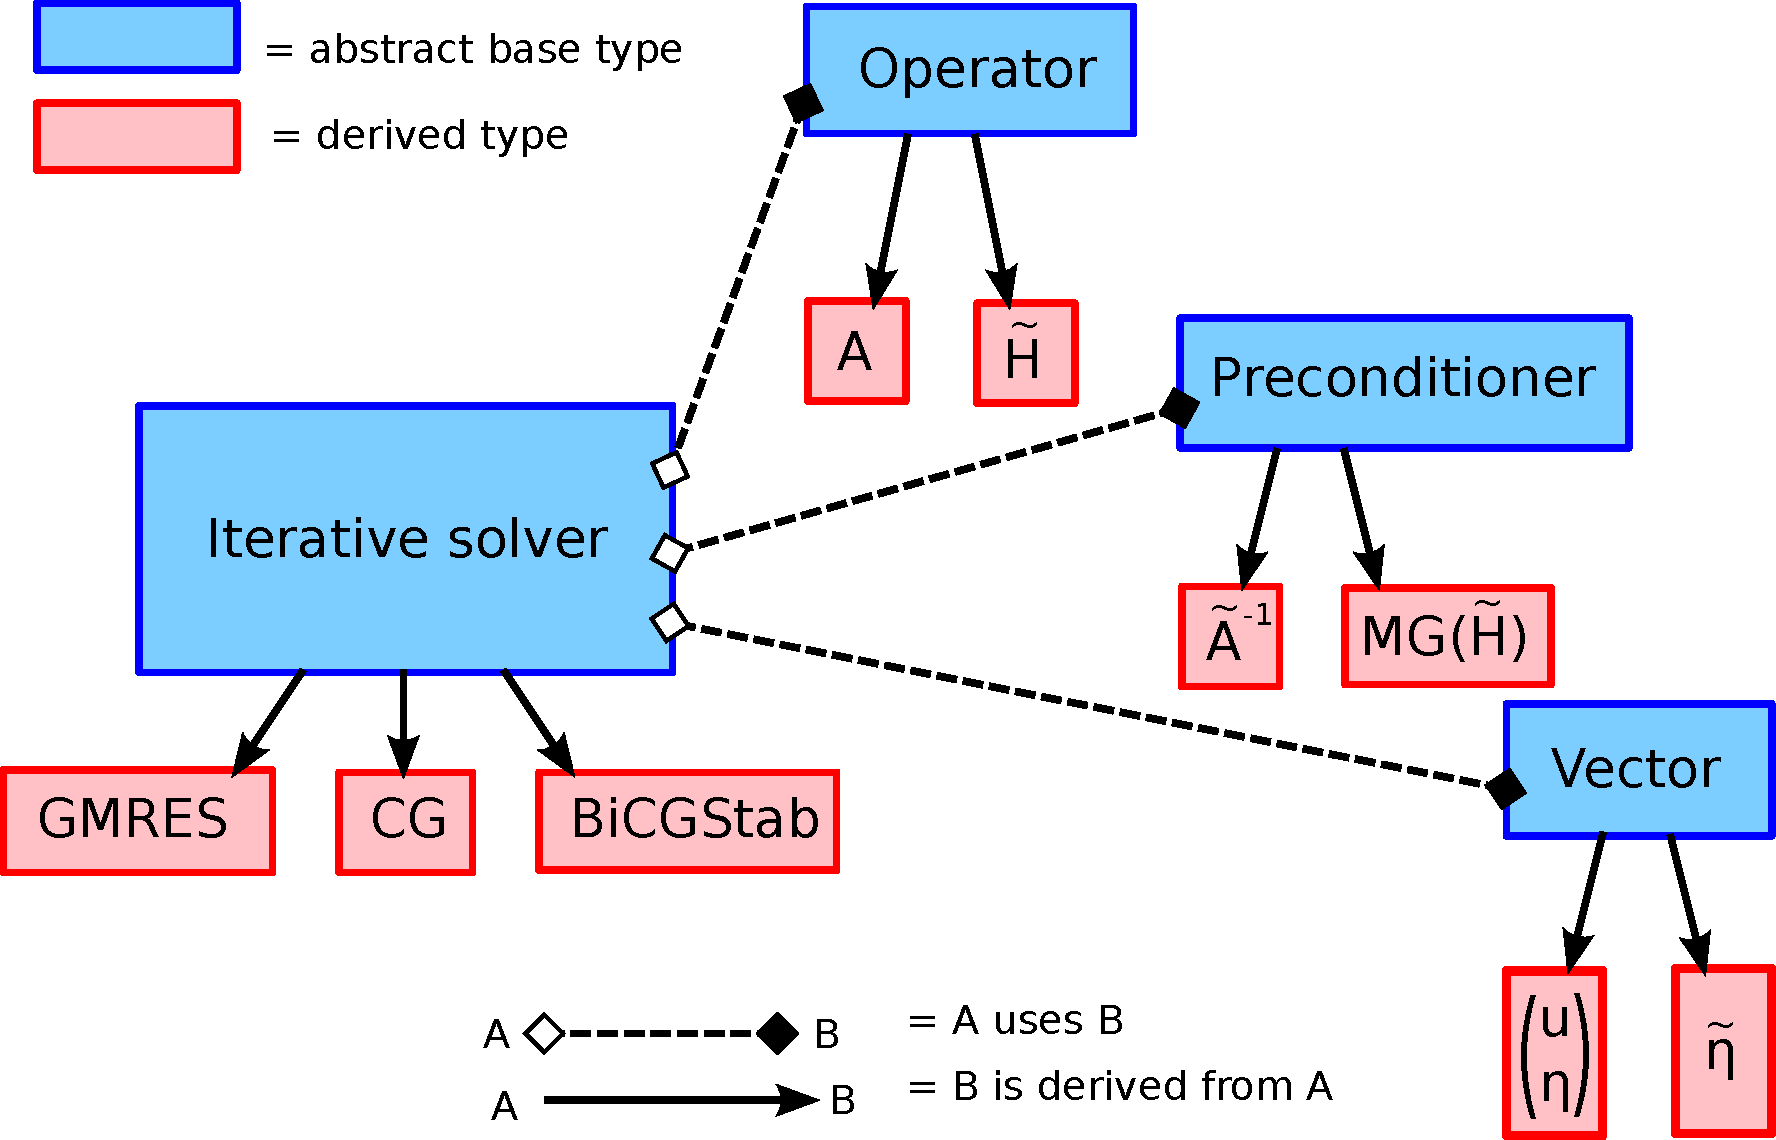
\includegraphics[width=0.45\linewidth]{Fig6a_class_hierarchy.pdf}
    \hfill
    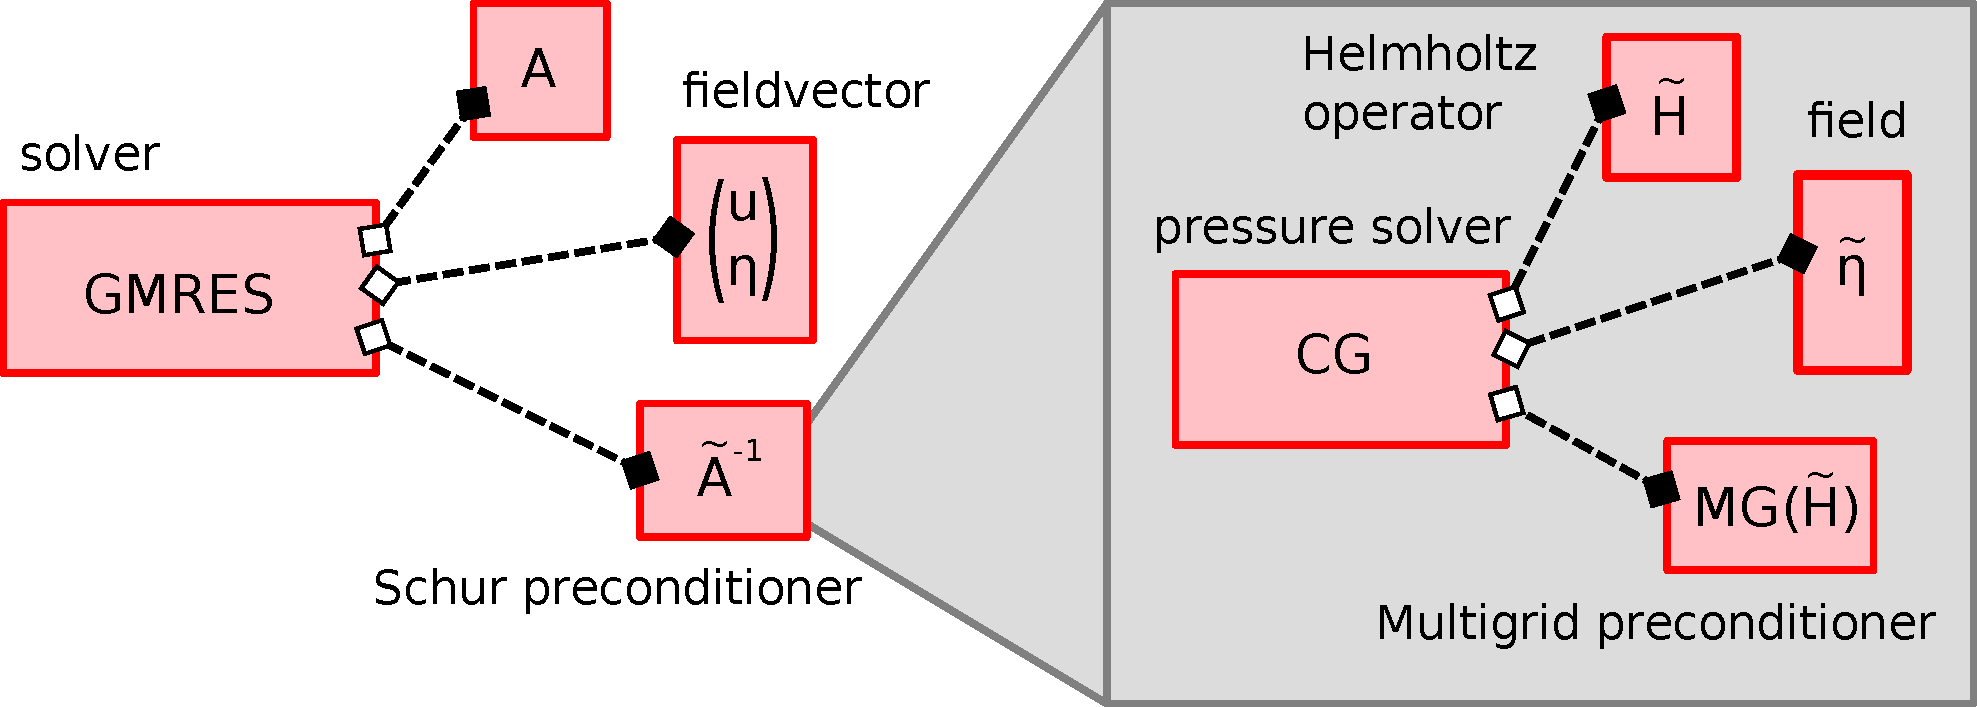
\includegraphics[width=0.45\linewidth]{Fig6b_class_concrete.pdf}
    \caption{Derived class hierarchy for solvers and preconditioners
      in LFRic (left) and concrete implementation for the linear
      system in implicit time-stepping (right).}
    \label{fig:class_hierarchy}
  \end{center}
\end{figure}
Each of those types is derived from an abstract base type. The
iterative solver types operate on generic vector types and are passed
preconditioner and linear operator objects which adhere to the
interface of their abstract base types.  This implies that only one
instance of a particular Krylov method has to be implemented in the
code. Apart from avoiding code duplication, this increases reliability
and maintainability, since only one instance of each solver has to be
developed and tested. In addition, it allows easy ``plug-and-play'' to
explore the space of all possible solver/preconditioner combinations
to achieve optimal performance.

To solve a particular problem, the user has to develop bespoke derived
types for the corresponding linear operator and preconditioners. Note
that the \texttt{apply()} methods of those derived types contain
invoke calls to kernels, which guarantees optimal performance of the entire
model. For example, to construct a solver for the implicit linear
system which is inverted in every semi-implicit time-step, the user
implements the following objects (see Fig.~\ref{fig:class_hierarchy},
right):
\begin{itemize}
\item A linear operator type which applies the full linear system to
  all components of a \texttt{field\_vector};
\item A preconditioner type which reduces the full linear system to
  the (approximate) Schur complement in pressure space by lumping the
  velocity mass matrix; this preconditioner then calls the solver for
  the pressure (Helmholtz-) system;
\item A linear operator type which applies the Helmholtz-operator for
  the pressure system;
\item A preconditioner type which approximately inverts the Helmholtz
  operator (see Subsection~\ref{sec:sub:preconditioner}).
\end{itemize}
Once implemented, those linear operators/preconditioners need to be
passed to suitable existing linear solvers.

In addition to this more traditional approximate Schur-complement
approach for solving the full linear system, the development of
solvers based on a hybridisation approach is currently being explored. Since
an exact Schur-complement can be formed in this case, hybridisation
avoids the expensive iteration over the full linear system, and
potentially leads to significant improvements in performance.

\subsection{\label{sec:sub:preconditioner}Preconditioner}

To precondition the strongly anisotropic Helmholtz-operator for the
pressure system, the tensor-product multigrid approach in~\cite{Borm2001} 
is being developed to use in LFRic. This is a more advanced solver than
the current tridiagonal vertical-only preconditioner in the ENDGame
model. The multigrid algorithm currently being developed in LFRic has been tested
extensively for representative elliptic equations in atmospheric
modelling in~\cite{Mueller2014,Dedner2016}, including a mixed-finite
element discretisation of a linear gravity wave system in~\cite{Mitchell2016}. 
The key idea to address the strong vertical
anisotropy due to the high-aspect ratio of the domain is to combine
vertical-only smoothing (line relaxation) with a horizontal multigrid
hierarchy. To allow the easy construction of the vertical-only
operators in the Schur-complement from the finite element
discretisation of the full equations, a suitable operator algebra was
developed in~\cite{Mitchell2016} and tested in the Firedrake
library. For horizontally discontinuous function spaces (such as the
pressure space, $Q_0^D$, and the vertical-only components of the $RT_0$ 
velocity space, see Subsection~\ref{sec:sub:spatial} for more details), 
operators can be assembled into a partially assembled matrix type, which 
stores all couplings within one vertical column. Matrices of this type can be
multiplied, added and, most importantly, inverted in the tridiagonal
solvers which realises the vertical line relaxation. This allows the
high-level construction of the building blocks required for the
Helmholtz-solver and preconditioner. The same data structures were
implemented as derived Fortran 2003 types in the LFRic code and form
the building blocks of the tensor-product multigrid preconditioner for
the elliptic Helmholtz system.


Compared to simpler preconditioners, which do not combine vertical
line relaxation with a horizontal multigrid hierarchy, the
tensor-product multigrid approach typically reduces the solution time
of the pressure system by a factor of at least two
~\cite{Mueller2014,Mitchell2016}. However, since the Helmholtz system
contains a zero-order term, only a small number ($\approx 3-4$) of
multigrid levels is required (independent of the grid
resolution). This greatly increases scalability since it avoids global
couplings which arise on the coarsest level.

\section{\label{sec:scal}Scaling}
The key performance metric for
LFRic and GungHo is scalability. The use of an unstructured mesh of
GungHo and the solver construction described in
Section~\ref{sec:Solver} should enable the LFRic model to scale to a
very large degree of parallelism. However, compiling some of the
Fortran 2003 OO constructs necessary to build such a solver
infrastructure is a challenging task for most compilers which has
delayed implementing such a solver. This remains a work in progress.

The February release of LFRic, named Dromedary, contains a simpler
solver. This employs a Krylov iterative algorithm, GCR on the mixed
system of velocity, potential temperature, density, exner
pressure. This is preconditioned by an approximate Schur complement
for the exner pressure which uses lumped mass matrices. The pressure
(Helmholtz) system is solved with BiCGstab and preconditioned by a
vertical only tridiagonal solver. Both mixed and helmholtz solvers use
a relative tolerance of $10^{-6}$.

\begin{figure}
  \begin{center}
    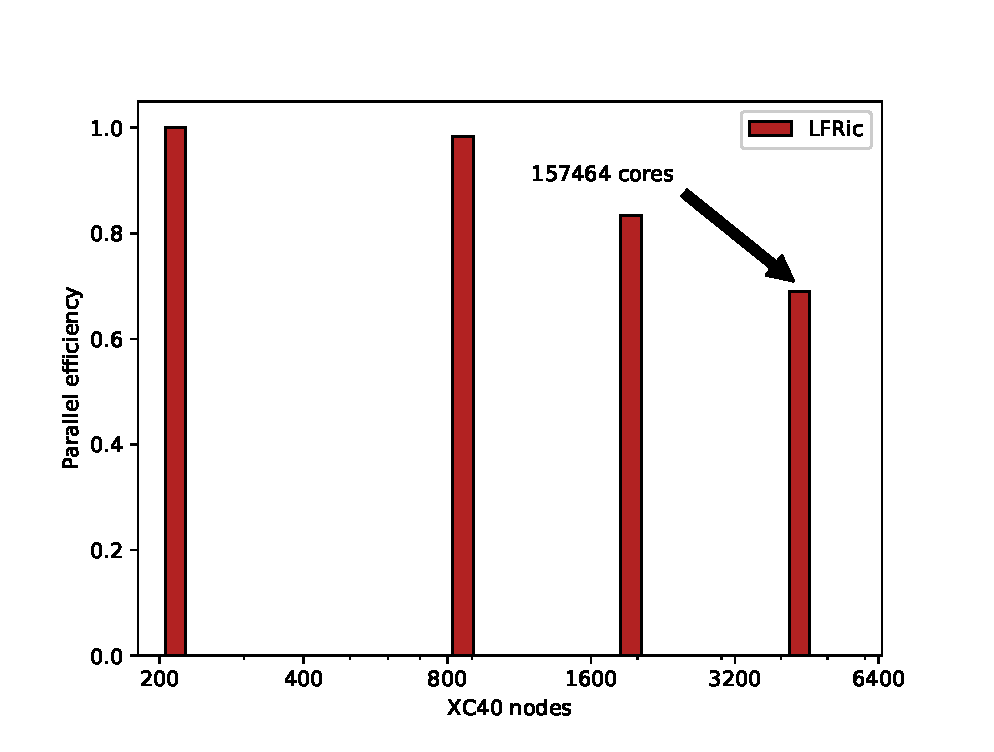
\includegraphics[width=0.85\linewidth]{Fig7_scale.eps}
    \caption{\label{fig:scale_PE}Strong scaling of the parallel efficiency of the LFRic 
      time-steps compared to 216 nodes. {\em N.B.} The x-axis shows a
      logarithmic scale}
  \end{center}
\end{figure}

Shown in Figure~\ref{fig:scale_PE} is 
the parallel efficiency of the LFRic time-step for a very high 
resolution model run. The mesh is a $C1944$ cubed-sphere with 30 
levels, where each panel has $1944 \times 1944$ cells. This roughly corresponds 
to a 5km global resolution. The science configuration is the baroclinic wave 
test~\cite{qj.2241} with a 75 second time-step. The code was compiled 
to production level (\verb+ -O3+) with the Intel17 compiler. The model 
was run in hybrid mode with both MPI and OpenMP on the Met Office Cray 
XC40. Each node comprises of dual socket Intel Xeon (Broadwell) 
18-core processors. The affinity was set to be three MPI ranks per 
socket with six OpenMP threads per MPI rank. 

The model shows good scaling out to a very large number of nodes,
$4374$, which is $157366$ cores. Scaling starts to drop off at this
scale to just below $70\%$ compared to $216$ nodes. Here, the local
volume has been reduced to $12\times 12$ with only $30$ levels that is
only $4320$ dofs per unit of parallelism for the pressure space. The
ratio of communication to computation cost will become worse if the
problem is scaled further. Moreover, the number of iterations for the
solver is relatively large and with multiple solves per time-step and
five global sums per iteration of the BiCGStab algorithm, means the
cost global sum becomes prohibitive.

The new solver implementation will enable better scaling by reducing
the number of Krylov solver iterations required by using a much more
efficient preconditioner. This will also reduce the absolute
performance, {\em i.e.} run-time. Further improvemnents are then
planned for computational optimisation once the solver is closer to
being algorithmically
optimal.

\begin{figure}
  \begin{center}
    \subfloat[]{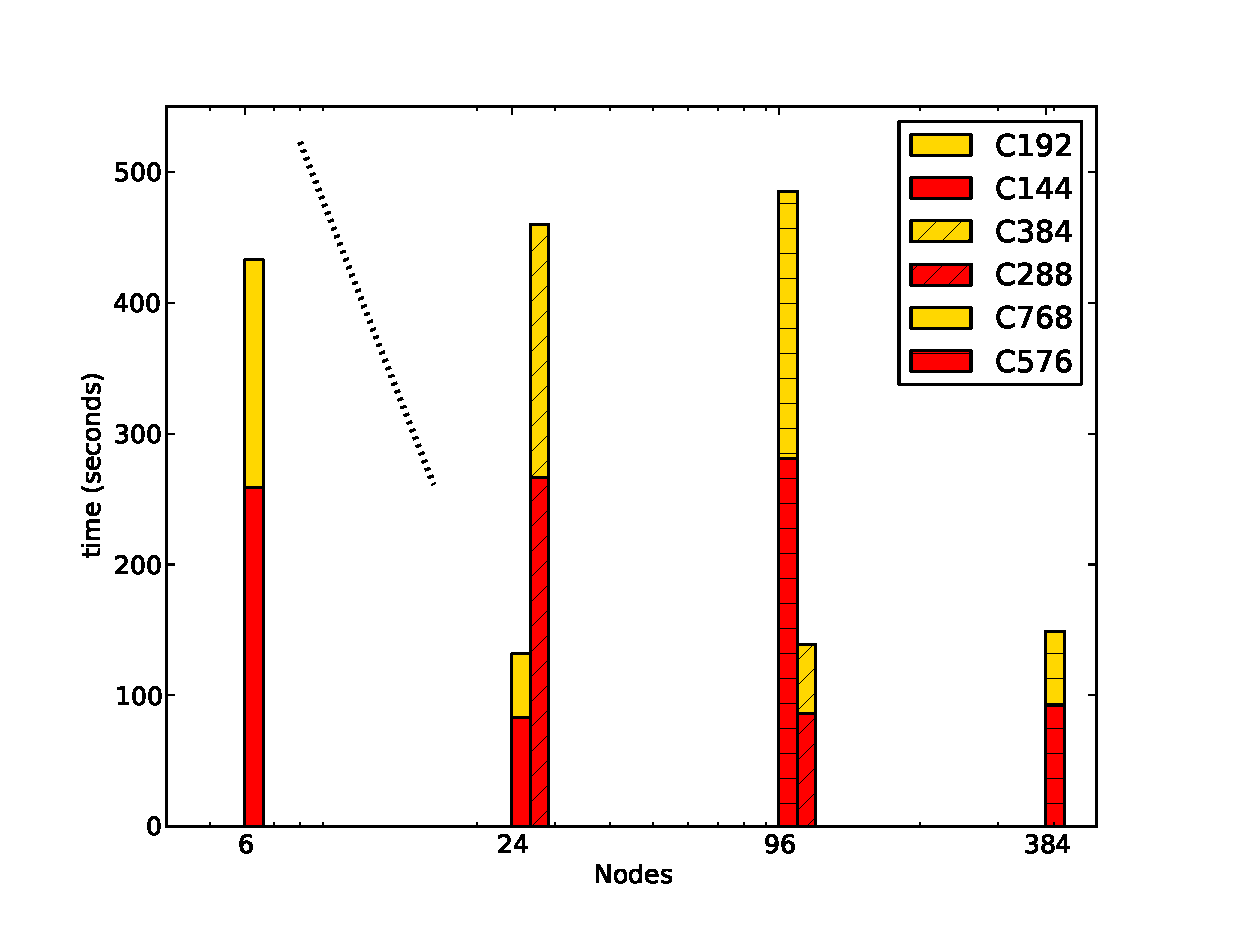
\includegraphics[width=0.75\linewidth]{Fig8a_strong_mv_T1.eps}}\\
    \subfloat[]{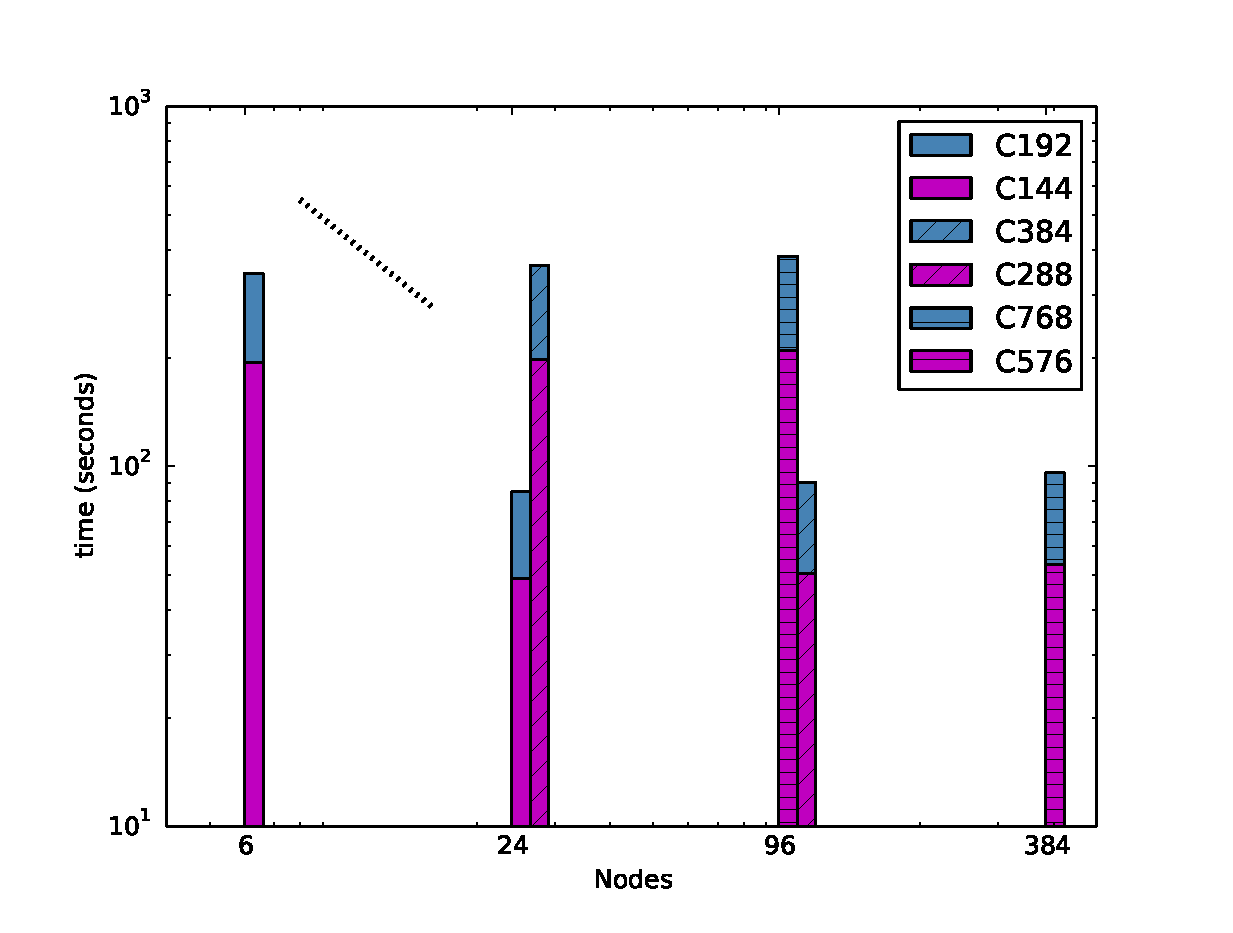
\includegraphics[width=0.75\linewidth]{Fig8b_strong_mv_T6.eps}}
    \caption{\label{fig:OMP_scale}Scaling of the matrix-vector routine
      run-time in seconds for $100$ time-steps, with different numbers
      of nodes for a) $18$ MPI ranks per socket and b) $3$ MPI ranks
      per socket and $6$ OpenMP threads per MPI rank. Same colour,
      same hatching shows strong scaling (the dashed line is to guide
      the eye), same colour diffent hatching shows weak scaling at
      different local volumes. The legend denotes the cubed-sphere
      mesh size.}
  \end{center}
\end{figure}

Shown in Figure~\ref{fig:OMP_scale} is the effect of using OpenMP on 
scaling for the matrix-vector routine. The data were produced using
the CrayPAT profiling tool on the Met Office Cray XC40. This was the
most expensive routine in the profile, as it is the dominant part of
the solver. The code was
again compiled with the Intel17 compiler. The model employs redundant
computation into the halos. Each processor computes the contribution
to dofs that reside on a shared mesh
entity (such as a face) which belong to a cell adjacent to a halo cell
from both the ``owned'' cell and the halo cell. Thus avoiding
comnuication that would otherwise be required to correctly calculate
the contribution of neighbour cells to that dof. Comparing MPI only to
the hybrid mode, each processor in the former regime has more work to
do in the case of redundant computation from the scaling of volume to
surface area. Hybrid mode has less cells to redundantly compute than
MPI only. Choosing redundant computation as a communication reduction
algorithm favours threading. Hence OpenMP is faster.
 

\section{Discussion and Conclusion}

The paper describes the novel features of the design of the new LFRic
model and infrastructure, and the GungHo dynamical core within it. In
short, the design has been developed and deployed successfully so
far. The GungHo dynamical core is routinely run in a range of
configurations. After initially being run in serial for many months
while the first version of PSyclone was developed, the introduction of
PSyclone enabled it to be run in parallel (both MPI and OpenMP) on
220,000 cores of a Cray XC40 within less than two weeks.

Several scientists are currently developing code within the
system. For the most part, scientists develop algorithms and kernels
within the existing infrastructure and with auto-generated PSy layer
code. For some newer developments the PSy layer code is hand-written
while new features are added to PSyclone. A clean separation between
the science code and the PSy layer code has been maintained
throughout. 

The need for PSyclone and the LFRic infrastructure to continuously
evolve in the light of new and changing science requirements
underlines an important point: the ``separation of concerns'' that has
enabled the science code to be kept isolated from the parallel systems
code does not mean that scientists and engineers can work in
isolation. In fact, the close ties between the scientists and software
engineers has been a key part of the success of the approach.

The compute performance of the dynamical core is promising. While
significant improvements in the algorithmic design are required to
deliver better throughput of the model, the application scales well to
160,000 cores. One of the first improvements to the algorithmic
performance is anticipated to come from application of the new solver
API discussed in the paper.

The design supports both MPI and OpenMP parallelism. The approach of
computing results into the halo redundantly so as to reduce
interprocessor communications helps the performance of deployments
with more OpenMP threads per MPI rank (for a given total core count)
because the larger domain of the high-thread runs means that the
relative size of the halos, and therefore the relative amount of
redundant computation, is smaller.

The overall design has sought to carefully modularise functionality. A
benefit of this is to enable trialling of different externally sourced
libraries. A benefit of this approach was seen when it was decided to
exchange the ESMF library for the YAXT library as the work was done in
a short period of time.

Development of the core LFRic infrastructure and PSyclone is still in
early days. LFRic is currently written to support any order of finite
element method on a range of different unstructured meshes. Should the
GungHo science converge on a particular mesh or set of meshes, and on
a particular FEM order it will likely be possible to refactor the
underlying LFRic data model to support more efficient access to the
data.

Largely, PSyclone is used to apply MPI and OpenMP. However its
features include the ability to add transformations that increase the
amount of redundant computation so as to reduce the number of halo
swaps, to re-order kernels and to loop-fuse kernels to provide a
performance benefit. Work is also underway to support OpenACC
transformations.

As well as continuing the technical capabilities of LFRic, currently,
sub-grid physics processes are being added to the GungHo dynamical
core implementation of LFRic with a view to steadily building up to a
fully-specified NWP model around 2020. Assuming the scientific and
computational performance results are acceptable it will likely go
head-to-head with the Met Office UM for 3-4 years while it is further
enhanced and optimised, eventually replacing the Unified Model
atmosphere at the core of the Met Office operations.

\label{sec:con}
\begin{itemize}
   \item It works! 
   \item single source science code
   \item target different programming models, MPI and OpenMP
   \item Shows good scaling
   \item Choice of alg (redundant computation - communication
     avoiding) means threading is favoured - OpenMP is faster
   \item Separation of concerns - modular design don't have to keep
     implementing over again during dev.
   \item e.g. Swap ESMF for YAXT
   \item more to come, solver, less global sums scale better
   \item Alg optimal -> also much faster
   \item then computational optimisation
   \item OpenACC progamming model for GPUs
   \item more Science, still single source.
   \item {\em Huzzah}
\end{itemize}
\newpage

\bibliography{mibib.bib}

\end{document}
